\documentclass[10pt]{article}

\usepackage{fullpage}
\usepackage[margin=2cm]{geometry}
\usepackage[pdftex]{graphicx}
\usepackage{float}

{{\ttfamily \hyphenchar\the\font=`\-}%

\begin{document}

\title{\vspace{-2cm}ARM11 Final Report}
\author{\small Alexander CLARKE, Qiang FENG, Jordan SPOONER, Laurence SQUIRES}

\maketitle

\section{ARM11 Emulator and Assembler}

The folder structure for the project is as follows:

\begin{itemize}
\item \texttt{src/} holds the \texttt{emulate.c} and \texttt{assemble.c} files, as well as files used by both emulate and assemble.
\item \texttt{src/emulate\_utils/} contains the files containing the constants, structs and helper functions used by emulate.
\item \texttt{src/assemble\_utils/} contains the files containing the constants, structs and helper functions used by assemble.
\end{itemize}

\subsection{Emulator Implementation}

See \texttt{doc/Checkpoint.pdf} for a brief overview of our implementation and \texttt{doc/LaTeX Documentation/refman.pdf} for full documentation.

\begin{figure}[H]
\begin{minipage}{0.4\linewidth}

\subsection{Assembler Implementation}

We structured our assembler as follows:

\begin{itemize}
\item \texttt{assemble.c} contains the function \texttt{main}, which takes two arguments. The first is a filename for a text file containing valid ARM11 assembly instructions. The second is a filename to which the assembled ARM11 binary object code is written. \texttt{main} is responsible for reading in the assembly instructions, tokenizing them using the helper functions in \texttt{tokenize.c}, creating a symbol table, assembling the tokenized input using the helper functions in \texttt{assembler.c}, and writing the object code to a binary file. It is also responsible for freeing any remaining allocated memory in order to avoid memory leaks.
\end{itemize}

\end{minipage}
\hspace{0.05\linewidth}
\begin{minipage}{0.55\linewidth}

\centering
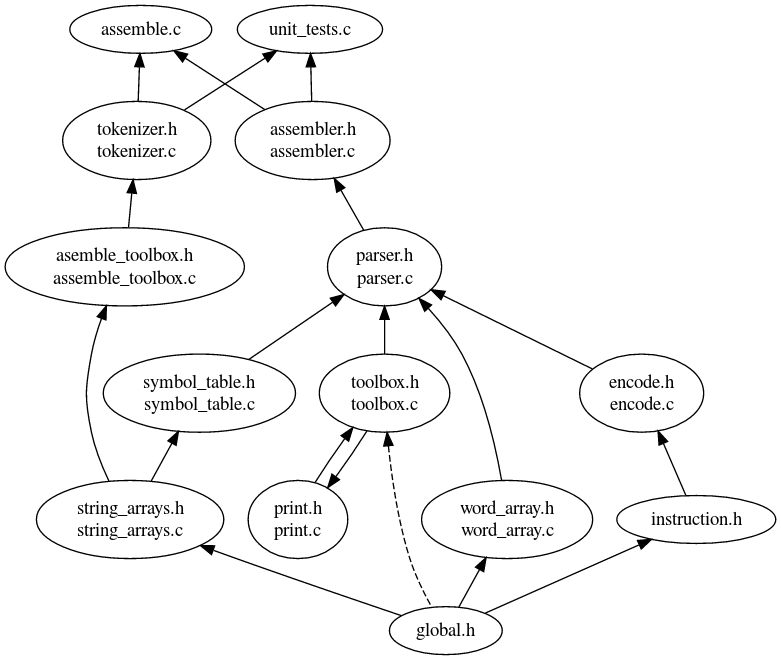
\includegraphics[scale=0.28]{Report/assemble.png}
\caption{Dependency Graph for \texttt{assemble.c}}

\end{minipage}
\end{figure}

\begin{itemize}
\item \texttt{unit\_tests.c} contains a simple test suite that uses assertions to check that called functions meet their documented functionality.
\item \begin{sloppypar}\texttt{tokenizer.c} contains the function \texttt{tokenize\_input} as well as several private helper functions. \texttt{tokenize\_input} creates an array of string arrays from the assembly input. Each string array represents a label or instruction. Each string array splits the instructions into its useful components, by removing and splitting around spaces and commas, and including any \texttt{[} and \texttt{]} characters seperately.\end{sloppypar}
\item \texttt{assemble\_toolbox.c} contains the functions \texttt{lines\_in\_file} and \texttt{load\_source\_file}, which are used by \texttt{assemble.c} to count the number of lines in the assembly file and then load the file, saving the input to a 2D array of characters. It also contains the function \texttt{save\_file}, used by \texttt{main} to write a binary file, and the functions \texttt{create\_2d\_array} and \texttt{free\_2d\_array}, which are used by \texttt{assemble.c} and \texttt{tokenizer.c} to create and free 2D character arrays.
\item \texttt{string\_arrays.c} defines the \texttt{string\_arrays\_t} struct. This is an expandable array of \texttt{string\_array\_t} structs. When initialised, the \texttt{string\_arrays\_t} struct can hold \texttt{INITIAL\_ARRAY\_LENGTH} string arrays, but the size is automatically reallocated and expanded when necessary. This file also defines the functions \texttt{make}, \texttt{add} and \texttt{free}. The \texttt{string\_arrays\_t} struct is used by \texttt{tokenizer.c} to break up the input into its useful parts. \texttt{string\_array.h} defines the \texttt{string\_array\_t} struct that simply holds an array of strings and the number of strings in that array.
\item \texttt{assembler.c} contains the function \texttt{assemble\_all\_instructions}, which is used by \texttt{main}'s second pass, in order to assemble the \texttt{string\_arrays\_t} of tokenized instructions to a \texttt{word\_array\_t} of assembled binary object code, given the symbol table of defined labels (which is generated in the first pass). It does this by calling one of five private helper functions, each of which assembles a single instruction of one of the five types. First, an \texttt{instruction\_t} representation of the current instruction is constructed, and this is then converted to a binary word by \texttt{encode.c}.
\item \texttt{parser.c} defines several helper functions used by \texttt{assemble.c}. In particular, it defines \texttt{string\_to\_mnemonic} which is used to convert a string of an operator to an enum, as well as similar functions for conditions, opcodes, addresses and shifts. It also defines the functions \texttt{parse\_shift} and \texttt{parse\_operand} which reads through operand tokens and updates the \texttt{instruction\_t} representation of the current instruction accordingly.
\item \texttt{encode.c} defines the \texttt{encode} function, which is called by \texttt{assembler.c}. It takes an \texttt{instruction\_t} representation of the current instruction, and returns the binary word that encodes that instruction. \texttt{instruction.h} defines the \texttt{instruction\_t} struct, which holds all of the information required to determine an instruction (see the documenation for emulate).
\item \texttt{symbol\_table.c} defines the \texttt{symbol\_table\_t} struct, which holds labels and their line numbers. It also contains the functions \texttt{generate\_symbol\_table} to generate a new symbol table from a tokenized assembly input, \texttt{get\_address} get the line number of a given label, and \texttt{free\_table} to free all allocated memory.
\item \texttt{word\_array.c} defines an expandable array of \texttt{word\_t} types, used to hold assembled instructions, as well as \texttt{make}, \texttt{add} and \texttt{free} functions.
\item \texttt{toolbox.c} includes several miscellaneous functions used throughout the code (see the documenation for emulate). 
\item \texttt{global.h} includes constants and type aliases which are used throughout the code (see the documenation for emulate).
\end{itemize}

See \texttt{doc/LaTeX Documentation/refman.pdf} for full documentation.

\subsection{Quality Assurance and Testing}

\subsubsection{Quality Assurance}

\paragraph{Style Guide}
Throughout the project, in order to ensure consistent styling in our code, we followed a style guide, which can be found at \texttt{doc/Style Guide.md}. We extensively discussed our proposed code style before writing any code. The style guide helped to make debugging much easier, by ensuring that the code reads easily, and making bugs easier to spot.

\paragraph{Code Reviews}
For each task allocated by the group, one team member was asked to review the code and sign it off. This meant that every block of code has been read by at least three team members: one who wrote the code, one who tested it, and one who signed it off. This process makes it exceedingly difficult to introduce bugs or poorly thought-out code.

\subsubsection{Testing}

\paragraph{Automated Testing}
Each time \texttt{make} is called, a script, \texttt{run\_quick\_tests} is called, which allows group members to continuously test their code as they write it. This runs \texttt{valgrind} on a few test cases, runs our unit tests, and then runs our extended ruby test suite. Most bugs can be spotted through this process. There is also a second script \texttt{run\_tests} that additionally runs \texttt{valgrind} on all test cases (which can take a few minutes), and clones the original ruby test suite seperately.

\paragraph{Unit Tests}
We have a C program, \texttt{unit\_tests.c} that runs through several assertions to check that our helper functions for \texttt{emulate} and \texttt{assemble} work as documented.

\paragraph{Memory Checks}
Any memory leaks, or use of uninitialized values will be shown by \texttt{valgrind} when our testing script is run.

\paragraph{Ruby Test Suite}
We extended the provided ruby test suite, with extra tests that are prepended with \texttt{new\_}. These extra test cases check cases which were not checked by the original test suite, as well as the extra shift functions that we have introduced.

\section{Terminal-based Motion-controlled Game Engine using OpenCV}

\subsection{Introduction}

Our group’s chosen extension comes in two parts. The first part is a versatile ASCII-graphics game engine. The second part is a hand tracking program built using OpenCV. Together they can be used to create simplified kinetic type game system. 

The game engine can be used to create many different 2D games. We created both flappy bird and snake to show its utility. The games can be controlled by keyboard or using our hand tracking program. Our hand tracking program uses a webcam to return the position of where it believes the hands are which would then be used by our game engine. Together they create an engaging game experience.

\subsection{Implementation}

\subsubsection{Terminal-based ASCII Game Engine}

\begin{itemize}
\item \texttt{ascii\_art.h}\footnote{Note that all these files are combined into one file when the game engine is used with the motion control due to difficulties with CMake.} contains the ASCII art struct, storing the ascii art, the colour, the height and the width.
\item \texttt{object\_list.h} contains the data struct that stores the state of the game, storing all objects and their state, such as velocity and acceleration.
\item \texttt{object\_list.c} contains functions for manipulating and using the object list. Using \texttt{new\_list} and \texttt{add\_elem} you create the initial state of the game. You can then use \texttt{for\_all} to apply any function, such as \texttt{move\_objects} which will update all objects position and acceleration accordingly. \texttt{free\_object\_list} is then used to free all memory used by the list at the end of the game.
\item \texttt{flappy\_bird.c} after using \texttt{init\_game} to create the initialised \texttt{object\_list}, repeated calls to \texttt{render\_game} will update the game state and then render the game. \texttt{bird\_coll} is used to determine whether you have died. To flap in the game you must call flap on the bird object. How this would work would be determined by whichever main you use.
\item \texttt{snake.c} contains the same sort of functions as \texttt{flappy\_bird}, but used for creating a snake game. \texttt{snake\_hit} is used instead of \texttt{bird\_coll} for for if the snake has died. When you call \texttt{render\_game} you must provide the new direction for the snake 
\item \texttt{main.c} calls the mentioned \texttt{flappy\_bird} functions, using space bar to flap. A different main file is used to use the game with the webcam.
\item \texttt{main\_snake.c} calls the mentioned snake functions, using WASD controls for the direction of the snake. A different main file is used to use the game with the webcam.
\end{itemize}

\subsubsection{Hand Tracking using OpenCV}

\begin{itemize}
\item \texttt{calibration.c} the main function \texttt{calibrate} is used to identify the range of colours to be used to identify the skin of the user. It does this by counting down while the user holds their hand up inside a highlighted box and then averaging the colour of each pixel present in the box and taking an appropriate range. This data is returned using the \texttt{calibration\_t} struct.
\item \texttt{detection.c} is used to detect the position of the user hands. It takes a thresholded image containing only the skin of the user and the last position of the hands. It then updates the position by moving the points away from the center and towards any high density region of skin, this is achieved by the loop repeatedly calling \texttt{apply\_force} and the returning the final position of the points once they have converged. The data containing the position of the hands is encoded in the \texttt{hands\_t} struct.
\item \texttt{main.cpp} contains the main logic for controlling the loop for the game. Initially it gets the webcam input and then calibrates the colour to the users skin, then it enters the loop that calculates if the user has flapped, updates the game and then renders the game until the user edits. Although it is a \texttt{cpp} file it is actually still C, the reason for it being \texttt{cpp} is to enable use of OpenCV since the headers for OpenCV are written for C++, however we still only call the legacy C functions.
\item \texttt{threshold.c} is used to threshold the image to the users skin colour. The function \texttt{get\_arm} takes the current frame (webcam image) and the calibration and then updates each pixel of the frame, making them white if it is detected as skin and black if not.
\item \texttt{uchar\_array.c} contains a struct for encoding lists of unsigned chars as well as functions to calculate the average and standard deviation of all the values in the list.
\end{itemize}

\subsection{Quality Assurance and Testing}

TODO.

\section{Project Evaluation}

\subsection{Group Working and Communication}

Our group initially came together to work out what structure our project would have. We then worked out all of the data types that we would need to implement our design for the structure and then implemented them. Using these, we came up with function prototypes.

Our group created a shared Google Docs spreadsheet to track all of the functions we thought we needed to implement. There were three jobs for each function. These were: complete the code, create unit tests for the code and review (and sign off) the code. We then assigned jobs to different team members, but sometimes we completed other people's jobs if it improved our groups workflow. Often we would implement functions inside different files to make version control easier.

We found that the most effective form of communication was always face-to-face, so we tried to spend as much time as possible in the Computing labs, where communication was easiest. At other times, we were able to continue working by using Slack and our shared spreadsheet.

Overall, our group worked well together. The communication and organisation between members in our group meant that we were always aware of what we should be doing, and also what other members were doing. We split up the work well, with all members of the team contributing fairly equally.

\paragraph{Benefits}
Our main benefit of our group organisation and communication is that we always knew what needed to be done, and we always knew that necessary functions would be created for us when we would need them. Thanks to our google spreadsheet and general communication it made our project more efficient and easier. We would definitely use this in our next project.

We would also definitely keep our group’s work ethic for the next project. We would all do a lot of coding which insured our project was easy to complete.

We would also keep our project structure of working in different files. This insured that we would not waste time with merge conflicts. While we did still have some merges, however, there weren’t too many. Our number of files also made it easier to find the function that you were searching for. 

\paragraph{Drawbacks}
We did run into some problems which we would like to avoid for next time. We initially were planning for our extension to be based upon a difficult to use, poorly documented robot. We wasted time trying to get it to work, and in the end decided to go for something that we were more certain would be possible to make. Next time we would try to insure that everything that we plan to use would have adequate documentation and tutorials if we are not familiar with it.

Another thing that we would change next time was preparing for the Lexis test instead of doing the project for so long. While obviously we needed to prepare for the test, we shouldn’t have not worked on the project for as long as we did. This meant that we were rushed for time toward the end of the project. While we still hit our internal (and external) deadlines, given more time we could have improved our extension and not as been as stressed.

Finally, we would try to spend more time in Computing labs, as it is much easier to work when everyone is present. In particular, it was often the case that only one or two group members would be present in the mornings, which restricted the amount of useful work we could do, and forced us to stay later in the evenings.

\subsection{Individual Reflections}

\paragraph{Alexander CLARKE}
I feel that our group worked very well together, myself included. As we all got along and contributed a good amount of work group organisation was very easy. If I was working with a different group of people I may have had to actively insure an efficient work environment, but this was not necessary in our group. 

My weakness for this project is probably my lack of experience with LaTeX, especially considering the number of marks awarded to the two reports. However, this was easily accommodated by my team with other group members doing the LaTeX editing. In a different group I may have had to learn LaTeX if there were no group members that had experience with it. Overall working with this group made our project far easier.

\paragraph{Qiang FENG}
I feel that I have integrated into the group very well. This is evidenced by the fact that I have received very high marks for both WebPA assessments, and comments often stated that I was a good team member.

Initially, I thought that my main strengths in the group would be my prior knowledge of git, my debugging skills and also my ability to work hard for long periods of time. I thought that my tendency to be pedantic about good and clean code style would be hard to live with, as I would have to work with code that other members have written.

As it turns out, my git knowledge was quite useful to other group members, and I sometimes had to help others when they had issues with git. Furthermore, my tendency to enforce good code style was also good for the group in general, as we could then understand each other's code much more easily - meaning we did not have to spend that long on our \texttt{emulate} and \texttt{assemble} programs.

Ultimately, my weakness in the group was the fact that I did not know C beforehand. However, I now feel that I am proficient in C, so if I was in a different group, I would be able to help others who may not know C that well. Also, I sometimes needed guidance from other team members to work out what I needed to do, even though we have the Google Spreadsheet which indicated what needed to be done. Although, since our team communicated with each other well, this was not that big of a problem.

If I had a different group, I would definitely maintain the active enforcement on good code style, as I feel that this aspect sped up development of our project. I would also try to be more proactive in working out what we needed to do since the members might not be as reliable as the ones in our current group.

\paragraph{Jordan SPOONER}
I am very happy with how our group has performed, and believe that, like all of our group members, I have made a significant contribution to our project: something which is backed up by my WebPA scores and feedback.

One of my strengths is organisation, and as such I have been making sure that our group has been making deadlines, such as for the checkpoint and the WebPA assessments, helping to assign tasks and keeping track of progress.

I pushed our team to spend the first week familiarising ourselves with the C language and carefully planning our project. Although there was some resentment amongst other group members, who wanted to start writing code as quickly as possible, I believe we made the right decision. The time we took to discuss our project structure, style, and high-level implementation details, and to learn C and assign tasks in the first week allowed us to complete both emulate and assemble by the end of the second week, and meant that unlike some other groups, there was no need to rewrite large blocks of code as we learnt more C or reached difficult parts of the project.

I also pushed our group to put a lot of emphasis on coding style, testing and documentation. Again, this was met with some resentment but I believe it made debugging a much easier, painless process, with very few bugs appearing, and debugging usually taking minutes instead of days, as was the case in some other groups. In particular, our unit tests made it easy to spot where bugs were being introduced in emulate, and allowed us to fix them easily.

My weakness is likely my lack of knowledge of some git functionality. Thankfully, Qiang and other group members were able to help answer my questions, and we avoided any git catastrophes. I didn't write as much code as some other group members, but I feel I made up for this by my contributions to planning, debugging, and to other parts of the project.

If I were in a different group, I would again push for planning and continuous testing. I believe these are the factors that contributed largely to the success of our project.

\paragraph{Laurence SQUIRES}
I feel I have integrated well into the group. My WebPA feedback reflects this and I am happy with the comments I received from members and the scores given. We have worked well as a team, finishing all our code within the time and to a high standard despite taking on a difficult extension. In addition, we have written extensive documentation and unit tests for the project, going beyond the specification and implementing features not included in the given test cases. 

Throughout the whole project my strengths have been in writing well structured modular code. Initially I did find it difficult to grasp the overall structure of our code, but after reading the specification properly and planning out how our code will work as a team we found designating tasks and working on them separately to the best approach. This approach worked well as we could focus on specific task, writing good code and unit tests for our functions and then later merging them with the help of others. This led to a quick completion of section one and two as well as all the optional test cases.

My biggest weakness in the project was definitely my knowledge of git: our project heavily utilised version control and I had to refer to teammates for help with understanding how git works and how to properly merge code after a merge conflict. However, throughout the course of our project I have learnt and now feel proficient in git having a good understanding of branches and merges. In addition, another weakness this project uncovered was my ability to write concise and understandable documentation. As the project was large with many different functions all being written by different members it was essential to have documentation for our functions. These comments explained what a function does as well as the parameters and return type, and they greatly helped when we had to combine our code to get a working system in the end.

If I had a different group, I would definitely maintain the style of management used in our group of designating specific functions and planning out the overall structure together. I would also try and write documentation and unit tests for functions before actually writing the functions code, as this might lead to more understandable code and easier debugging of the larger system.

\end{document}
